\documentclass[11pt]{article}
\usepackage{fullpage}
\usepackage{amsthm}

\usepackage{amsthm,amsmath,amsfonts,amssymb,amstext,enumitem}
\usepackage{latexsym,ifthen,url,rotating,graphicx}
\usepackage{listings}
\usepackage{tikz}
\usetikzlibrary{arrows,shapes,positioning,fit}
\usepackage{graphicx}
\usepackage[font=small,labelfont=bf]{caption}



% --- -----------------------------------------------------------------
% --- Document-specific definitions.
% --- -----------------------------------------------------------------
\lstset{
    columns=fixed,
    literate={—}{{---}}1 {…}{{...}}1
}

\newcommand{\todo}[1]{{\color{red}[TODO:{#1}]}}

\newtheorem{problem}{Problem}
\newtheorem{corollary}{Corollary}
\newtheorem{fact}{Fact}
\newtheorem{exercise}{Exercise}
\newtheorem{theorem}{Theorem}
\newtheorem{definition}{Definition}
\newtheorem{notation}{Notation}
\newtheorem{lemma}{Lemma}
\newtheorem{example}{Example}

\newcommand{\getsr}
  {{\:\stackrel{\raisebox{-2pt}{${\scriptscriptstyle \hspace{0.2em}\$}$}}
   {\leftarrow}\:}}
\newcommand{\points}[1]{\textbf{({#1} pts)}}

\newcommand{\fn}{\footnotesize}
\newcommand{\Colon}{\ : \ }
\newcommand{\st}{\mathsf{state}}
\newcommand{\msgs}{\mathcal{M}}
\newcommand{\ctxts}{\mathcal{C}}
\newcommand{\keys}{\mathcal{K}}
\newcommand{\rands}{\mathcal{R}}
\newcommand{\states}{\mathcal{S}}
\newcommand{\kg}{\mathcal{K}}
\newcommand{\Enc}{\mathsf{Enc}}
\newcommand{\Dec}{\mathsf{Dec}}
\newcommand{\MAC}{\mathrm{Mac}}
\newcommand{\Vrfy}{\mathrm{Vrfy}}
\newcommand{\RMAC}{\mathrm{RMAC}}
\newcommand{\tags}{\mathcal{T}}
\newcommand{\testeq}{\stackrel{?}{=}}
\newcommand{\win}{\mathsf{win}}
\newcommand{\leng}{\mathsf{len}}

\newcommand{\pk}{pk}
\newcommand{\sk}{sk}

\newcommand{\calD}{\mathcal{D}}
\newcommand{\calA}{\mathcal{A}}
\newcommand{\calE}{\mathcal{E}}
\newcommand{\calB}{\mathcal{B}}
\newcommand{\AES}{\mathsf{AES}}

\newcommand{\algorithm}[1]{\textbf{Alg} {#1}}

\newcommand{\calO}{\mathcal{O}}

\newcommand{\dlog}{\mathrm{dlog}}

\newcommand{\Adv}{\mathbf{Adv}}
\newcommand{\AdvPRF}[2]{\Adv^{\mathrm{prf}}_{#1}({#2})}
\newcommand{\AdvPRG}[2]{\Adv^{\mathrm{prg}}_{#1}({#2})}
\newcommand{\AdvCPA}[2]{\Adv^{\mathrm{cpa}}_{#1}({#2})}
\newcommand{\AdvCCA}[2]{\Adv^{\mathrm{cca}}_{#1}({#2})}
\newcommand{\AdvKR}[2]{\Adv^{\mathrm{kr}}_{#1}({#2})}
\newcommand{\AdvCKR}[2]{\Adv^{\mathrm{ckr}}_{#1}({#2})}
\newcommand{\AdvRMR}[2]{\Adv^{\mathrm{rmr}}_{#1}({#2})}
\newcommand{\AdvCR}[2]{\Adv^{\mathrm{cr}}_{#1}({#2})}
\newcommand{\AdvUFCMA}[2]{\Adv^{\textrm{uf{-}cma}}_{#1}({#2})}
\newcommand{\AdvDL}[2]{\Adv^{\mathrm{dl}}_{#1}({#2})}

\newcommand{\Exp}{\mathbf{Exp}}
\newcommand{\ExpOW}[1]{\Exp^{\mathrm{ow}}({#1})}
\newcommand{\ExpCKR}[2]{\Exp^{\mathrm{ckr}}_{#1}({#2})}
\newcommand{\ExpRMR}[2]{\Exp^{\mathrm{rmr}}_{#1}({#2})}

\newcommand{\concat}{{\,\|\,}}
\newcommand{\xor}{\oplus}
\newcommand{\bits}{\{0,1\}}

\newcommand{\tcolh}{T^{\mathrm{col}}_h}
\newcommand{\tcolH}{T^{\mathrm{col}}_{H^2}}
\newcommand{\Hcomb}{H^{1\|2}}
\newcommand{\Hxor}{H^{1\oplus2}}

\newcommand{\EXP}{\textrm{EXP}}
\newcommand{\MODEXP}{\textrm{MOD{-}EXP}}
\newcommand{\ADD}{\textrm{ADD}}
\newcommand{\MULTIMODEXP}{\textrm{MULTI{-}MOD{-}EXP}}
\newcommand{\MUL}{\textrm{MUL}}
\newcommand{\MOD}{\textrm{MOD}}

\newcommand{\GG}{\mathbb{G}}
\newcommand{\ZZ}{\mathbb{Z}}

\newcommand{\bK}{\mathbf{K}}
\newcommand{\bof}{\mathbf{f}}
\newcommand{\bU}{\mathbf{U}}
\newcommand{\bM}{\mathbf{M}}
\newcommand{\bC}{\mathbf{C}}

\newcommand{\rvrange}{\mathcal{R}}
\newcommand{\rspace}{\mathcal{C}}

\newcommand{\hatalpha}{\hat{\alpha}}
\newcommand{\hatb}{\hat{b}}
\newcommand{\hatc}{\hat{c}}
\newcommand{\hatt}{\hat{t}}
\newcommand{\hatm}{\hat{m}}

\newcommand{\barm}{\overline{m}}

\newcommand{\otp}{\mathrm{OTP}}
\newcommand{\des}{\mathrm{DES}}
\newcommand{\twodes}{\mathrm{2DES}}
\newcommand{\threedes}{\mathrm{3DES}}
\newcommand{\threedestwo}{\mathrm{3DES2}}
\newcommand{\aes}{\mathrm{AES}}
\newcommand{\pad}{\mathsf{pad}}
\newcommand{\unpad}{\mathsf{unpad}}
\newcommand{\Func}{\mathrm{Func}}
\newcommand{\cbcmacpad}{\mathsf{pad}_{\mathrm{cbc}}}


\newcommand{\Img}{\mathrm{Im}}

\newcommand{\Expt}{\mathbf{Expt}}
\newcommand{\ExptCPA}{\mathbf{Expt}^{\mathrm{cpa}}}
\newcommand{\ExptCCA}{\mathbf{Expt}^{\mathrm{cca}}}
\newcommand{\ExptOTCPA}{\mathbf{Expt}^{\mathrm{1\mbox{-}cpa}}}
\newcommand{\ExptOTCPAone}{\mathbf{Expt}^{\mathrm{1\mbox{-}cpa\mbox{-}1}}}
\newcommand{\ExptOTCPAzero}{\mathbf{Expt}^{\mathrm{1\mbox{-}cpa\mbox{-}0}}}
\newcommand{\AdvOTCPA}[2]{\Adv^{\mathrm{1\mbox{-}cpa}}_{#1}({#2})}
\newcommand{\ExptCPAone}{\mathbf{Expt}^{\mathrm{cpa\mbox{-}1}}}
\newcommand{\ExptCPAzero}{\mathbf{Expt}^{\mathrm{cpa\mbox{-}0}}}
\newcommand{\ExptUF}{\mathbf{Expt}^{\mathrm{uf}}}
\newcommand{\AdvUF}[2]{\Adv^{\mathrm{uf}}_{#1}({#2})}

\newcommand{\LR}{\mathrm{LR}}

\newcommand{\Piotp}{\Pi_\mathrm{otp}}
\newcommand{\Encotp}{\Enc_\mathrm{otp}}
\newcommand{\Decotp}{\Dec_\mathrm{otp}}
\newcommand{\bhat}{\hat{b}}
\newcommand{\dict}{\mathtt{dict}}
\newcommand{\Col}{\mathsf{Col}}
% --- -----------------------------------------------------------------
% --- Lecture notes formatting macros
% --- -----------------------------------------------------------------

%
% The following commands set up the lecnum (lecture number)
% counter and make various numbering schemes work relative
% to the lecture number.
%
\newcounter{lecnum}
%\renewcommand{\thepage}{\thelecnum-\arabic{page}}
\renewcommand{\thesection}{\thelecnum.\arabic{section}}
\renewcommand{\theexercise}{\thelecnum.\arabic{exercise}}
\renewcommand{\theexample}{\thelecnum.\arabic{example}}
\renewcommand{\thedefinition}{\thelecnum.\arabic{definition}}
\renewcommand{\theequation}{\thelecnum.\arabic{equation}}
\renewcommand{\thefigure}{\thelecnum.\arabic{figure}}
\renewcommand{\thefact}{\thelecnum.\arabic{fact}}
\renewcommand{\thetable}{\thelecnum.\arabic{table}}


%
% The following macro is used to generate the header.
%
\newcommand{\lecture}[2]{
   %\pagestyle{myheadings}
   %\thispagestyle{plain}
   \newpage
   \setcounter{lecnum}{#1}
   \setcounter{page}{1}
   \noindent
   \begin{center}
   \framebox{
      \vbox{\vspace{2mm}
    \hbox to 6.28in { {\bf CMSC 28400 Introduction to Cryptography
                        \hfill Autumn 2020} }
       \vspace{4mm}
       \hbox to 6.28in { {\Large \hfill #2 \hfill} }
       \vspace{2mm}
       \hbox to 6.28in { {\it Instructor: David Cash} \hfill }
      \vspace{2mm}}
   }
   \end{center}
   %\markboth{Lecture #1: #2}{Lecture #1: #2}
   \vspace*{4mm}
}





% --- -----------------------------------------------------------------
% --- The document starts here.
% --- -----------------------------------------------------------------
\begin{document}
%\lecture{**LECTURE-NUMBER**}{**DATE**}{**LECTURER**}{**SCRIBE**}
\lecture{11}{Notes \#11: Message Authentication}

%\tableofcontents

So far we've been concerned with secrecy of messages, and have considered
ciphers and randomized encryption with various secrecy security goals.  These
notes consider a different security goal: \emph{authenticity of messages}.
Intuitively, we'd like tools that help prevent adversaries from changing or
inserting messages on communications links. A typical setting is a compromised
connection on the internet, where an untrusted router controls all of the
messages being sent. Another setting is a cell connection, where an adversary
with a powerful antenna may interfere with traffic between a device and a cell
tower. While in those settings secrecy is also a goal, we're going to focus
exclusively on authenticity first, and then return to how it may combined with
secrecy.

\subsection{Message Authentication Codes (MACs)}

Let us start with an abstract setting. A sender and receiver are connected via
a channel that is controlled by an adversary $\calA$ who may change their
messages (See Figure~\ref{fig:channel}). If the endpoints don't
share \emph{something}, then there's not much they can do: The bits arriving at
the receiver could just as well have come from the sender as the adversary.  So
we'll assume, like we did with encryption, that the two endpoints share a key
$k$, and that they'll try use $k$ to somehow stop $\calA$, who doesn't know
$k$.

A first idea might be to encrypt $m$ using a cipher or randomized encryption
scheme, and send $c$ instead. The receiver could then decrypt and consider the
output as the received message. (See Figure~\ref{fig:encchannel}.)
Assuming encryption is secure (say many-time CPA secure), does this ensure that
when $\hatm$ is received, it was really sent by the sender?  The answer is ``not
always'' (at least). This is because \emph{malleability attacks} may be
possible, where an adversary can change the contents of a ciphertext even when
it does not know the key. Whether or not the change is meaningful is a separate
issue, but we can say with confidence that sometimes $\calA$ may sneak in
a $\hatm$ that wasn't actually sent.

\begin{figure}[h]
\begin{center}
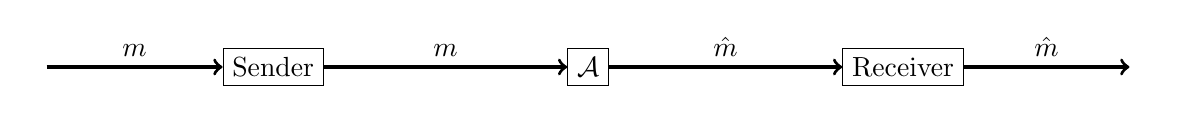
\begin{tikzpicture}
    \tikzset{vertex/.style = {shape=rectangle,draw,align=center}}
    \tikzset{edge/.style = {->,very thick}}
    % vertices
    \node[vertex] (1) at  (0,0) {Sender};
    \node[vertex] (2) at  (4,0) {$\calA$};
    \node[vertex] (3) at  (8,0) {Receiver};
    \node (4) at  (-3,0) {};
    \node (5) at  (11,0) {};
    \draw[edge] (4) -- (1) node[midway,above]  {$m$};
    \draw[edge] (3) -- (5) node[midway,above]  {$\hatm$};
    \draw[edge] (1) -- (2) node[midway,above]  {$m$};
    \draw[edge] (2) -- (3) node[midway,above]  {$\hatm$};
\end{tikzpicture}
\end{center}
    \caption{An unprotected channel.}
    \label{fig:channel}
\end{figure}

\begin{figure}[h]
\begin{center}
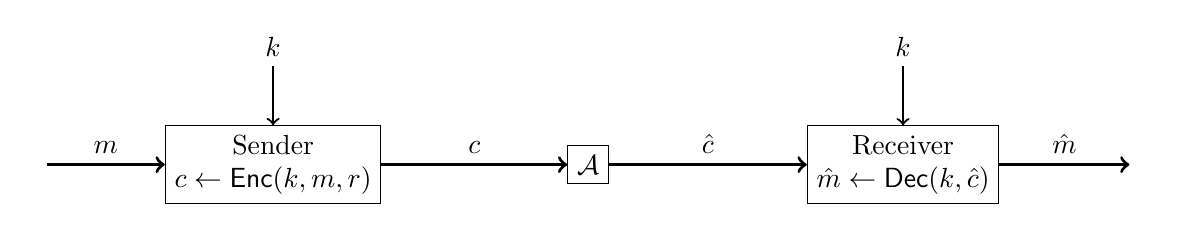
\begin{tikzpicture}
    \tikzset{vertex/.style = {shape=rectangle,draw,align=center}}
    \tikzset{edge/.style = {->,very thick}}
    % vertices
    \node[vertex] (1) at  (0,0) {Sender\\ $c\gets\Enc(k,m,r)$};
    \node[vertex] (2) at  (4,0) {$\calA$};
    \node[vertex] (3) at  (8,0) {Receiver\\ $\hatm\gets\Dec(k,\hatc)$};
    \node (4) at  (0,1.5) {$k$};
    \node (5) at  (8,1.5) {$k$};
    \node (6) at  (-3,0) {};
    \node (7) at  (11,0) {};
    \draw[edge] (6) -- (1) node[midway,above]  {$m$};
    \draw[edge] (3) -- (7) node[midway,above]  {$\hatm$};
    \draw[edge] (1) -- (2) node[midway,above]  {$c$};
    \draw[edge] (2) -- (3) node[midway,above]  {$\hatc$};
    \draw[->,thick] (4) -- (1); 
    \draw[->,thick] (5) -- (3); 
\end{tikzpicture}
\end{center}
    \caption{An attempt at authentication
    using encryption.}
    \label{fig:encchannel}
\end{figure}


Instead of trying to use encryption schemes for authentication, we're going to
define a new primitive, called a \emph{message authentication code} (MAC) that
is purpose-built.  The term MAC is very standard, to the point where we almost
never call them by the full name, so we'll just say MAC everywhere below.

Our plan to prevent messages changes is to require that all received messages
be accompanied by a \emph{tag}. A tag is a just a message-specific bitstring,
which intuitively should only be computable by the sender who knows the secret
key $k$. For security, we want that it should be hard to ``forge'' a tag
when someone doesn't know the key.

We start with a definition, which is very simple.
\begin{definition}
    A function 
    \begin{align*}
        \MAC  : \keys\times\msgs  \to  \tags 
    \end{align*}
    is called a \emph{MAC} with key-space $\keys$, message-space $\msgs$,
    and tag-space $\tags$.
\end{definition}
This doesn't say anything about security, but the names at least guide usage
(see Figure~\ref{fig:macchannel}).  The idea is that the endpoints share a
random $k\in\keys$.  When they want to send a message $m\in\msgs$, they compute
$t\gets\MAC(k,m)$ and send $m$ and $t$ together.  Upon receiving some (possibly
modified) message and tag pair $(\hatm,\hatt)$, the receiver checks if the tag
is correct, meaning it checks if $\hatt \testeq \MAC(k,\hatm)$. If not, then it
throws an error, and otherwise it accepts $\hatm$ as authentic.

\begin{figure}[h]
\begin{center}
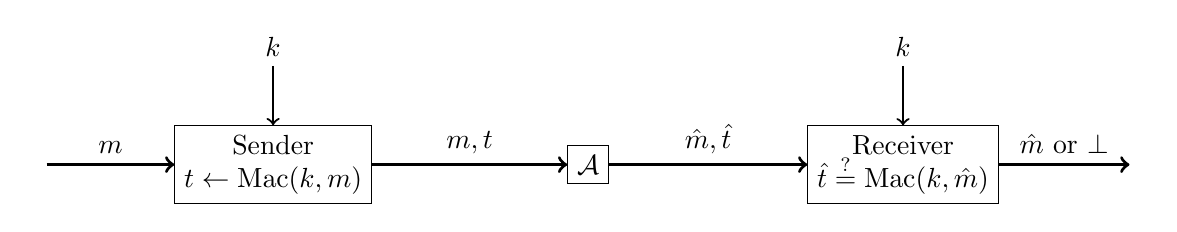
\begin{tikzpicture}
    \tikzset{vertex/.style = {shape=rectangle,draw,align=center}}
    \tikzset{edge/.style = {->,very thick}}
    % vertices
    \node[vertex] (1) at  (0,0) {Sender\\ $t\gets\MAC(k,m)$};
    \node[vertex] (2) at  (4,0) {$\calA$};
    \node[vertex] (3) at  (8,0) {Receiver\\ $\hatt \testeq \MAC(k,\hatm)$};
    \node (4) at  (0,1.5) {$k$};
    \node (5) at  (8,1.5) {$k$};
    \node (6) at  (-3,0) {};
    \node (7) at  (11,0) {};
    \draw[edge] (6) -- (1) node[midway,above]  {$m$};
    \draw[edge] (3) -- (7) node[midway,above]  {$\hatm$ or $\bot$};
    \draw[edge] (1) -- (2) node[midway,above]  {$m,t$};
    \draw[edge] (2) -- (3) node[midway,above]  {$\hatm,\hatt$};
    \draw[->,thick] (4) -- (1); 
    \draw[->,thick] (5) -- (3); 
\end{tikzpicture}
\end{center}
    \caption{A channel protected with a MAC.}
    \label{fig:macchannel}
\end{figure}

Before going further, let's stop to note one attack that we won't prevent: if
$\calA$ observes a message/tag pair $m,t$ being sent, then later it can
\emph{replay} this pair by sending it again. In our diagram above there's
nothing the MAC can do stop this, since it really is the correct $t$. Thus
we'll have to deal with replay attacks by changing the message we send, or
by other means like timestamps in the messages themselves.

\subsection{MAC Security: Unforgeability}

It's clear that we need some security property from MAC in order for it
to do any good. We'd like to somehow say that producing a tag for a message
is hard if you don't know the key. As with our encryption definitions, we've
going to think ``worst case''. Namely, we'll want the following properties
of a security definition:
\begin{enumerate}
    \item An adversary is trying to win an experiment by ``forging'' a tag
        on a message.

    \item We'll declare an adversary to have won if it can produce a tag on
        \emph{any} message $\hatm\in\msgs$ that was not tagged by the sender.
        It doesn't matter if $\hatm$ is ``meaningful'' or not (because we
        can't formalize this; what's meaningful will depend on the application).

    \item We won't count replay attacks as winning, for the reasons discussed
        above.

    \item We'll assume that the adversary can observe several message/tag
        pairs to help it try to forge a tag. In practice these examples come
        from some protocol run by the endpoints.
        In our worst-case thinking, we'll let $\calA$ pick these example
        messages to be tagged. That way, no matter protocol the endpoints
        run, we'll have confidence that forging is hard.

    \item We'll assume that the adversary can try injecting messages and see
        if the receiver rejects the tags or not. In practice an adversary
        can often tell whether or not a server rejects a message, so the
        definition will give the ability explicitly.
\end{enumerate}
With those points in mind, here's the definition.
\begin{definition}
    Let $\MAC  : \keys\times\msgs  \to  \tags$
    and let
    $\calA$ be an algorithm. Define algorithm $\ExptUF_F(\calA)$ as
    \begin{center}
    \begin{tabular}{c}
        \begin{minipage}{2in}\begin{tabbing}
            123\=123\=\kill
            \underline{\algorithm{$\ExptUF_F(\calA)$}} \\[2pt]
            \fn01 \> Pick $k\getsr \keys$\\
            \fn02 \> Run $\calA^{\MAC(k,\cdot),\Vrfy_k(\cdot,\cdot)}$, where
            the second oracle is given below. \\
            \fn03 \> If $\calA$ ever queried $\Vrfy(\cdot,\cdot)$ on an
            input $(\hatm,\hatt)$ such that \\
            \> \> (1) $\hatt = \MAC(k,\hatm)$, and \\
            \> \> (2) $\hatm$ was not previously queried to the first oracle,\\
            \> then output $1$.\\
            \fn04 \> Else: Output 0\\
            \\
            \underline{Oracle $\Vrfy_{k}(\hatm,\hatt)$} \\[2pt]
            \> If $\hatt = \MAC(k,\hatm)$: Return 1 \\
            \> Else: Return $0$
        \end{tabbing}\end{minipage}
    \end{tabular}
    \end{center}
    Define the \emph{unforgeability advantage of $\calA$ against $\MAC$} as
    \[
        \AdvUF{\MAC}{\calA} =
        \Pr[\ExptUF_\MAC(\calA) = 1].
    \]
\end{definition}
Fortunately for us, we'll only need one security definition for MACs this
quarter. 

The $\MAC(k,\cdot)$ oracle in the experiment gives the adversary the
ability to look at whatever tag it wants. The second oracle
$\Vrfy_k(\cdot,\cdot)$ serves two purposes: First, the adversary can probe it
to see if a message/tag pair is acceptable to the receiver. Second, it uses
this oracle to win the game, but submitting a message/tag pair $\hatm,\hatt$
that counts as a \emph{forgery}, meaning that $\hatm$ was not previously tagged
by the first oracle and yet $\calA$ cooked up an acceptable tag anyway.
The rationale for these oracle follows the desired features we listed before
the definition.


To solve the next exercise, use the ideas from the CCA notes to mount a
malleability attack, but phrase it in terms of an $\calA$ that fits the
syntax of the unforgeability experiment.
\begin{exercise}
    Let $\MAC:\bits^\ell\times\bits^\ell\to\bits^\ell$ be the $\ell$-bit
    one-time page ($\MAC(k,m)=k\oplus m$). Give a simple adversary issuing
    one query to each oracle such that $\AdvUF{\MAC}{\calA}=1$.
\end{exercise}

\subsection{Constructing a Fixed-Length MAC}

The exercise above gives a non-example of a MAC. Fortunately for us, there's a
simple relationship between PRFs and MACs, given by the next theorem. Note that
in the statement of the theorem, we refer to a function $F$ as being used in
both the PRF distinguishing experiment \emph{and} the unforgeability
experiment. This makes formal sense, since the syntax of $F$ fits either
definition, so we can measure the security of $F$ as either a MAC or a PRF.
\begin{theorem}
    Let $F  : \keys\times\msgs  \to  \tags$ and let $\calA$ be an
    algorithm. Then there exists an algorithm $\calB$, running about
    the same time as $\calA$, such that
    \[
        \AdvUF{F}{\calA} \leq \AdvPRF{F}{\calB} + \frac{q_v}{|\tags|},
    \]
    where $q_v$ is the number of times $\calA$ queries its $\Vrfy$ oracle.
    Moreover, $\calB$ issues the same number of queries as (the sum total number
    issued by) $\calA$.
\end{theorem}
\begin{proof}
    Fix $F$ and an adversary $\calA$ as stated in the theorem.  Build $\calB$
    as follows:
    \begin{center}
    \begin{tabular}{c}
        \begin{minipage}{2in}\begin{tabbing}
            123\=123\=123\=\kill
            \underline{Adversary $\calB^{\calO(\cdot)}$ \emph{//$\calO=F(k,\cdot)$ or $f$}}\\[2pt]
            \> Initialize an empty set $S$ \\
            \> Initialize a flag variable $\win\gets 0$\\
            \> Run $\calA$. Answer its oracle queries as follows:\\
            \> \> On query for $\MAC(k,m)$:\\
            \> \> \> Add $m$ to $S$\\
            \> \> \> Query $t \gets \calO(m)$. \\
            \> \> \> Return $t$ to $\calA$.\\
            \> \> On query for $\Vrfy_k(\hatm,\hatt)$:\\
            \> \> \> Query $t \gets \calO(\hatm)$. \\
            \> \> \> If $\hatt = t$ and $\hatm\notin S$: Set the flag $\win\gets 1$ and Return $1$\\
            \> \> \> Else If $\hatt = t$ and $\hatm\in S$: Return $1$\\
            \> \> \> Else: Return $0$\\
            \> When $\calA$ halts, output the flag $\win$
        \end{tabbing}\end{minipage}
    \end{tabular}
    \end{center}
    Let's unwrap what $\calB$ is doing. It has access to an oracle that either
    is either $F(k,\cdot)$ or a random function, and its goal is determine
    which. Its plan is to simulate the unforgeability experiment for $\calA$,
    and observe if $\calA$ ever wins the simulated experiment. Formally, if the
    oracle of $\calB$ is $F(k,\cdot)$ then the experiment will be properly
    simulated for $\calA$, and thus $\calA$ will win the simulation with
    probability $\AdvUF{F}{\calA}$. On the other hand, we're going to show that
    if the oracle is a random function $f$, then $\calA$ can win the simulated
    experiment with probability at most $q_v/|\tags|$. This latter probability is
    intuitively a union bound on guessing a tag blindly in $q_v$  tries.

    To complete the proof we calculate the advantage of $\calB$. First we
    claim that
    \[
        \Pr[\calB^{F(\bK,\cdot)}=1] = \Pr[\ExptUF_F(\calA)=1].
    \]
    This is true because if we plug in $F(\bK,\cdot)$ everywhere for $\calO$ in
    the description of $\calB$, then $\calB$ becomes \emph{exactly} the same
    algorithm as $\ExptUF_F(\calA)$.
    
    Next we prove that
    \[
        \Pr[\calB^{\bof(\cdot)}=1] \leq \frac{q_v}{|\tags|}.
    \]
    By definition, $\calA$ issues $q_v$
    queries to its $\Vrfy$ oracle. For $i=1,\ldots,q_v$, define 
    $W_i$ to be the event that the $\win$ flag is set to $1$ on the $i$-th
    query. If $\calB^{\bof(\cdot)}=1$, then definitely one of the $W_i$
    occurs (and vice versa). So we have
    \[
        \Pr[\calB^{\bof(\cdot)}=1] = \Pr[\bigcup_{i=1}^{q_v} W_i] \leq
        \sum_{i=1}^{q_v}\Pr[W_i].
    \]
    The inequality is just a union bound. We're going to show that $\Pr[W_i]
    \leq 1/|\tags|$ for all $i$, which will give
    \[
        \Pr[\calB^{\bof(\cdot)}=1] \leq
        \sum_{i=1}^{q_v}\Pr[W_i] \leq \frac{q_v}{|\tags|}.
    \]
    Finally the theorem is proved by simply rearranging the terms in the
    definition of the advantages of $\calA$ and $\calB$.

    Now for the bound $\Pr[W_i]\leq 1/|\tags|$. This holds because the only way
    for $W_i$ to happen is for $\calA$ to ``predict'' the value $\bof(\hatm)$
    without previously querying $\hatm$. But when $\hatm$ is not queried, the
    value $\bof(\hatm)$ is independent of the view of $\calB$ so far, and hence
    its guess $\hatt$ is independent of $\bof(\hatm)$. But $\bof(\hatm)$ is
    uniform, so the probability that $\hatt = \bof(\hatm)$ is $1/|\tags|$, as
    desired.
\end{proof}
One can intuitively sum up the relation between MAC and PRF security as: MAC
security is about \emph{predicting} a function $F$ on a point before you query
it. But if the output space $\tags$ is large, and you can predict a function
like that, then you must actually be distinguishing it from a random function!

Given a MAC that is secure for more than one message block is quite hard
(this is in contrast to randomized encryption, where something simple like CTR
mode is easy to state and not too hard to analyze). The next exercise shows
that some simple attempts don't work.
\begin{exercise}
    Let $\AES$ be the 128-bit AES block cipher as usual. Consider
    $F_1:\keys\times\msgs\to\tags_1$ and $F_2:\keys\times\msgs\to\tags_2$, with
    $\keys = \bits^{128}$, $\msgs=\bits^{128}\times\bits^{128}$,
    $\tags_1=\bits^{256}$, and $\tags_2=\bits^{128}$, defined by
    \begin{align*}
        F_1(k,m_1\|m_2) & = \AES(k,m_1)\|\AES(k,m_2),\\
        F_1(k,m_1\|m_2) & = \AES(k,m_1)\oplus\AES(k,m_2).
    \end{align*}
    Give a simple adversaries $\calA_1,\calA_2$ such that 
    $\AdvUF{F_1}{\calA_1}=1$
    and 
    $\AdvUF{F_2}{\calA_2}=1$.
\end{exercise}

\begin{exercise}
    The bound in the theorem becomes trivial if $q_v \geq |\tags|$. Intuitively,
    why should this be the case?
\end{exercise}

\subsection{CBC-MAC} 

In practice, something called CBC-MAC is often used for multi-block messages.
We won't even attempt to analyze it, as the proof is a bit too complicated. But
it's worth knowing in case you ever come across it. Here is the code: It takes
message-space $\msgs$ consisting of strings of at most $2^{128}-1$ bits long;
This is almost, but not quite, infinite, and is just a technical condition. The
key-space and tag-space are $\keys=\tags=\bits^{128}$. The construction works
as follows:
\begin{center}
        \begin{minipage}{2in}\begin{tabbing}
            123\=123\=\kill
            \underline{\algorithm{$\MAC(k,m)$}} \\[2pt]
            \> Let $\leng\in\bits^{128}$ be the bit-length of $m$, encoded
            as a $128$-bit integer.\\
            \> $\barm \gets \cbcmacpad(m)$\\
            \> Parse $\barm[1]\|\cdots\|\barm[L]\gets\barm$  \emph{($128$-bit
            blocks)}\\
            \> $v \gets \leng$ \\
            \> For $i=1,\ldots,L$: \\
            \> \> $v \gets \aes(k,v\oplus\barm[i])$\\
            \> Output $v$
        \end{tabbing}\end{minipage}
    \end{center}
The padding function $\cbcmacpad$ here is different from the PKCS padding we
saw before (I'm not sure why, actually). Luckily, $\cbcmacpad$ is simple:
it just appends a $1$ bit followed by the required number of zero bits to
get the resulting output to be a multiple of $128$ bits long.

As the name suggests,
CBC-MAC is similar to CBC encryption. The main differences are that 
\begin{enumerate}

    \item CBC-MAC is  deterministic. Instead of randomness, the first
        block is set to an encoding of the length.

    \item Only the final value of $v$ is output. Outputting the intermediate
        values of $v$ results in an insecure MAC (a good exercise!). You can
        check this even for messages such that $L=2$.

\end{enumerate}


\begin{exercise} 

    Consider a version of CBC-MAC where the length block is not used.  More
    precisely, define $\MAC_0$ to be exactly like $\MAC$ above, change the line
    just before the ``for'' loop to $v\gets 0^{128}$ instead of $v\gets\leng$.
    Give a simple $\calA$ such that $\AdvUF{\MAC_0}{\calA}=1$.  (Hint: A single,
    one-block query to $\MAC_0(k,\cdot)$ is enough.  The simplest attack I can
    think of then forges a tag on a two-block message $\hatm$.)
    This shows that we can't simply ignore then length block!

\end{exercise}

\begin{exercise}
    Requiring the length block at the start of the message is annoying,
    since it means you can't start processing until you know many bits
    you're sending. It'd be nice if we could move the length block
    to the end, but unfortunately this makes it insecure!

    Concretely, give a simple attack against the following MAC:
    \begin{center}
        \begin{minipage}{2in}\begin{tabbing}
            123\=123\=\kill
            \underline{\algorithm{$\MAC(k,m)$}} \\[2pt]
            \> Let $\leng\in\bits^{128}$ be the bit-length of $m$, encoded
            as a $128$-bit integer.\\
            \> $\barm \gets \cbcmacpad(m)$\\
            \> Parse $\barm[1]\|\cdots\|\barm[L]\gets\barm$  \emph{($128$-bit
            blocks)}\\
            \> $v \gets 0^\ell$ //start with zeros instead of length\\
            \> For $i=1,\ldots,L$: \\
            \> \> $v \gets \aes(k,v\oplus\barm[i])$\\
            \> $v \gets \aes(k,v\oplus\leng)$ // length block last\\
            \> Output $v$
        \end{tabbing}\end{minipage}
    \end{center}
\end{exercise}


\end{document}

